\PassOptionsToPackage{hyphens}{url}
\documentclass[10pt,a4paper]{article}

\usepackage[a4paper,margin=0.9in]{geometry}
\usepackage{fontspec}
\defaultfontfeatures{Ligatures=TeX}
% XeLaTeX/Overleaf setup:
% Upload these files into a `fonts/` folder in your Overleaf project.
%
% Core body font:
%   fonts/GillSans.ttf
%   fonts/GillSans-Bold.ttf
%   fonts/GillSans-Italic.ttf
%   fonts/GillSans-BoldItalic.ttf
%
% Optional fonts for a closer match to the sample PDF:
%   fonts/CoolveticaRg-Regular.ttf   % title
%   fonts/SegoeUI.ttf                % affiliation/email block
%   fonts/FolioBT-Light.ttf          % alternative affiliation block
%
% Body font: Gill Sans if uploaded or installed, otherwise a sans fallback that
% exists in the TeX environment.
\IfFileExists{fonts/GillSans.ttf}{
  \setmainfont[
    Path=fonts/,
    Extension=.ttf,
    UprightFont=*,
    BoldFont=*-Bold,
    ItalicFont=*-Italic,
    BoldItalicFont=*-BoldItalic
  ]{GillSans}
}{
  \IfFontExistsTF{Gill Sans}{
    \setmainfont{Gill Sans}
  }{
    \IfFontExistsTF{TeX Gyre Heros}{
      \setmainfont{TeX Gyre Heros}
    }{
      \setmainfont{Helvetica}
    }
  }
}

% Fallback font switches.
\newcommand{\TitleFont}{\bfseries\sffamily}
\newcommand{\AuthorFont}{\bfseries\sffamily}
\newcommand{\MetaFont}{\sffamily}
\newcommand{\HeadingFont}{\bfseries\sffamily}

% Optional title font, closer to the sample title treatment.
\IfFileExists{fonts/CoolveticaRg-Regular.ttf}{
  \newfontfamily\PaperTitleFace[Path=fonts/]{CoolveticaRg-Regular.ttf}
  \renewcommand{\TitleFont}{\PaperTitleFace}
}{}

% Prefer Gill Sans Bold for headings/authors when the bold face is uploaded.
\IfFileExists{fonts/GillSans-Bold.ttf}{
  \newfontfamily\PaperHeadingFace[Path=fonts/]{GillSans-Bold.ttf}
  \renewcommand{\HeadingFont}{\PaperHeadingFace}
  \renewcommand{\AuthorFont}{\PaperHeadingFace}
}{}

% Optional affiliation/details font, closer to the sample PDF.
\IfFileExists{fonts/FolioBT-Light.ttf}{
  \newfontfamily\PaperMetaFace[Path=fonts/]{FolioBT-Light.ttf}
  \renewcommand{\MetaFont}{\PaperMetaFace}
}{
  \IfFileExists{fonts/SegoeUI.ttf}{
    \newfontfamily\PaperMetaFace[Path=fonts/]{SegoeUI.ttf}
    \renewcommand{\MetaFont}{\PaperMetaFace}
  }{}
}
\usepackage{amsmath,amssymb}
\usepackage{graphicx}
\usepackage{booktabs}
\usepackage{array}
\usepackage{tabularx}
\usepackage{enumitem}
\usepackage{caption}
\usepackage{titlesec}
\usepackage{setspace}
\usepackage{natbib}
\usepackage{xurl}
\usepackage[hidelinks]{hyperref}

\setlength{\parindent}{0pt}
\setlength{\parskip}{0.16em}
\linespread{1.00}
\emergencystretch=1.5em
\raggedbottom
\captionsetup{font=small,labelfont=bf}
\setlist[itemize]{leftmargin=1.4em,topsep=0.2em,itemsep=0.2em}

\titleformat{\section}
  {\centering\HeadingFont\bfseries\normalsize}
  {\thesection}{0.7em}{}
\titlespacing*{\section}{0pt}{0.7em}{0.25em}

\titleformat{\subsection}
  {\HeadingFont\bfseries\normalsize}
  {\thesubsection}{0.6em}{}
\titlespacing*{\subsection}{0pt}{0.5em}{0.2em}

\titleformat{\subsubsection}[runin]
  {\HeadingFont\itshape}
  {\thesubsubsection}{0.5em}{}[.]
\titlespacing*{\subsubsection}{0pt}{0.35em}{0.3em}

\bibpunct{(}{)}{;}{a}{,}{,}
\setlength{\bibsep}{0pt}

\newcommand{\figsource}[1]{\caption*{\footnotesize\textit{Source: #1.}}}
\newcommand{\tabsource}[1]{\caption*{\footnotesize\textit{Source: #1.}}}

\begin{document}
\pagestyle{plain}

\begin{center}
{\TitleFont\fontsize{20}{24}\selectfont Digital Inclusion and Circular Economy Behavior in Indian States: A Digital Circularity Index and Explainable XGBoost Analysis\par}
\vspace{0.45cm}
{\AuthorFont\large\bfseries Suresh Kumar Chelliah, Shreya Srivastava and Yash Chauhan\par}
\vspace{0.1cm}
{\MetaFont\normalsize Department of Computational Intelligence, SRM Institute of Science \& Technology, Kattankulathur, Tamil Nadu, India\par}
{\MetaFont\normalsize sureshkc@srmist.edu.in; ss1371@srmist.edu.in; yc0810@srmist.edu.in\par}
\end{center}

\textbf{Abstract:} India's digital build-out and circular-economy agenda are often discussed in separate policy spaces: one in terms of broadband, mobile access and platform payments, the other in terms of waste, resource efficiency and environmental performance. At the state level, however, both transitions depend on a shared capacity to collect data, coordinate services and make resource flows visible. This paper asks whether states with stronger digital access also show stronger circular-economy behavior. Using seven official and policy-relevant data sources, we compile a harmonised dataset for 16 Indian states and construct three indicators: the Digital Access Score (DAS), the Circular Economy Behavior Score (CEBS) and the Digital Circularity Index (DCI). The analysis combines descriptive comparison, ordinary least squares regression, rank-based and permutation-based checks, mediation and threshold testing, leak-free nested cross-validation, SHAP-based explainability and K-Means clustering. The association is consistent but is interpreted cautiously. DAS and CEBS are positively related ($r=0.781$, $p<0.001$), and the result remains visible under alternative inference checks. Tele-density carries more explanatory weight than UPI adoption, which does not mediate the main relationship. This suggests that digital inclusion cannot be reduced to payment activity alone. Nested leave-one-out cross-validation gives XGBoost the strongest leak-free result ($R^2=0.511$), while clustering separates digitally stronger states from states where both digital and circularity indicators remain weaker. We read these findings as evidence of linked development capacity, not as proof of causality. For Indian policy, the practical implication is that connectivity, reporting systems and circular-economy administration should be planned together, especially in states where foundational capacity is weakest.

\textbf{Keywords:} circular economy; digital circularity index (DCI); digital inclusion; explainable machine learning; Indian states; XGBoost

\section{Introduction}

India's digital transition is now visible in everyday administration and commerce. Monthly UPI transactions exceed 14 billion \citep{npci2025}, national tele-density remains above 85\% \citep{trai2024}, and the Digital India programme has pushed broadband and mobile services into a wide range of regional settings. A second transition is unfolding at the same time. India is under pressure to manage e-waste, urban waste and resource-use inefficiency, while national policy institutions increasingly treat circularity as part of long-term growth strategy \citep{cpcb2023,nitiCE2021}.

The overlap matters because both agendas rely on more than technology adoption. Digital systems help only when they improve reporting, reach and coordination; circular-economy programmes also need reliable information about collection, processing and resource movement. Yet research on digital inclusion in India still concentrates mainly on access, payments and growth \citep{meity2023}, while circular-economy research tends to focus on waste systems, environmental governance and industrial transition \citep{geissdoerfer2017}. State-level evidence connecting the two remains thin. This paper builds a Digital Circularity Index from seven public data sources and tests whether digitally stronger states also perform better on selected circular-economy indicators.

The study evaluates three hypotheses. H1 states that states with higher Digital Access Scores will also have higher CE Behavior Scores. H2 asks whether UPI adoption acts as the channel between digital access and CE behavior. H3 tests whether CE behavior changes more sharply after a tele-density threshold.

\section{Literature Review}

Digital inclusion in India has advanced rapidly, but not evenly. Tele-density and digital payments have expanded across the country, yet large gaps remain between higher-capacity states and states with weaker infrastructure or lower income levels \citep{trai2024,npci2025}. Recent subnational work makes the same point: Indian states are moving through digitalisation at different speeds, with some states combining broad access and balanced use while others still face foundational constraints \citep{icrier2025}. Much of the policy literature treats these developments as routes to financial inclusion, efficiency and service access \citep{meity2023}. ICT-for-development scholarship is broader. It argues that digital systems also reshape governance, information flows and institutional capacity, which means their effects may extend into environmental management and sustainability outcomes \citep{avgerou2010,heeks2017}.

Circular-economy research points to a similar implementation problem. The concept has moved from global advocacy into Indian policy planning, especially through NITI Aayog's sector-based framework \citep{emf2013,nitiCE2021}. Even so, formal e-waste processing remains limited, state performance varies, and SDG-linked outcomes still differ substantially \citep{cpcb2023,nitiSDG2024}. Recent work on digital technologies and CE also places emphasis on information functions: generating data, tracking product origins, supporting resource management and making material loops easier to manage \citep{schoggl2023}. Taken together, these strands suggest a plausible connection. States with stronger digital access may be better positioned to coordinate reporting, traceability and circular-economy behavior. This paper tests that possibility directly.

\section{Methodology}

\subsection{Research design and data}

The study uses a cross-sectional design based on 16 Indian states with complete observations across all selected inputs. Because the sources do not cover every state in the same way, the sample is deliberately conservative: we keep only states that are comparable across every source and prioritise traceability over sample size. The final dataset combines nine raw and six derived variables, and Table~\ref{tab:data_sources_24} lists the core source variables.

\begin{table}[htbp]
\centering
\caption{Data Sources and Core Variables}
\label{tab:data_sources_24}
\small
\begin{tabularx}{\textwidth}{@{}>{\raggedright\arraybackslash}p{3.0cm}>{\raggedright\arraybackslash}X>{\raggedright\arraybackslash}p{1.5cm}@{}}
\toprule
\textbf{Source} & \textbf{Variable} & \textbf{Year} \\
\midrule
TRAI & Tele-density (\%) & 2024 \\
RBI & Per capita NSDP (INR) & 2023--24 \\
NITI Aayog & SDG Index Score & 2023--24 \\
NPCI/Dataful Insights & UPI transactions per capita & 2024--25 \\
CPCB & E-waste processed (tonnes) & 2021--22 \\
Census of India & Literacy rate (\%) & 2011 \\
Census of India & Urban population (\%) & 2011 \\
\bottomrule
\end{tabularx}
\tabsource{Compiled by the authors from official public datasets}
\end{table}

\subsection{Composite index construction}

To keep the index construction transparent, each raw variable is first rescaled to a 0--100 range using min--max normalisation:
\begin{equation}
\hat{x}_i=\frac{x_i-x_{\min}}{x_{\max}-x_{\min}}\times 100
\end{equation}

The Digital Access Score is defined as:
\begin{equation}
DAS = 0.40\hat{T}_d + 0.30\hat{U}_{pc} + 0.30\hat{N}_{pc}
\end{equation}
where $\hat{T}_d$ is tele-density, $\hat{U}_{pc}$ is UPI transactions per capita and $\hat{N}_{pc}$ is per capita NSDP after normalisation.

The Circular Economy Behavior Score is defined as:
\begin{equation}
CEBS = 0.35\hat{E}_{pc} + 0.40S_{sdg} + 0.25\hat{N}_{pc}
\end{equation}
where $\hat{E}_{pc}$ is normalised e-waste processed per capita and $S_{sdg}$ is the SDG Index score. The Digital Circularity Index then combines both dimensions multiplicatively:
\begin{equation}
DCI=\frac{DAS \times CEBS}{100}
\end{equation}

\subsection{Analytical strategy}

H1 is tested using a bivariate OLS model of CEBS on DAS, followed by HC3 robust errors, permutation tests, bootstrap intervals and rank-based correlations. H2 is assessed using the Baron and Kenny mediation framework with a Sobel test \citep{baron1986}. H3 is examined through piecewise regression with grid-searched breakpoint selection. Predictive stability is checked first with leave-one-out cross-validation and then with a stricter nested leave-one-out design. The machine-learning step is used as a stress test of the pattern rather than as a claim of operational forecasting accuracy. XGBoost is interpreted using SHAP values \citep{lundberg2017}, and K-Means clustering is used to identify state typologies.

\section{Results and Discussion}

\subsection{Descriptive patterns}

The first pattern is simple: DCI is not spread evenly across the sample. Haryana records the highest DCI (72.97), Karnataka posts the highest DAS (94.40), and Bihar ranks lowest across all three composite indicators. Figure~\ref{fig:dci_ranking_24} shows the state-level spread.

\begin{figure}[htbp]
\centering
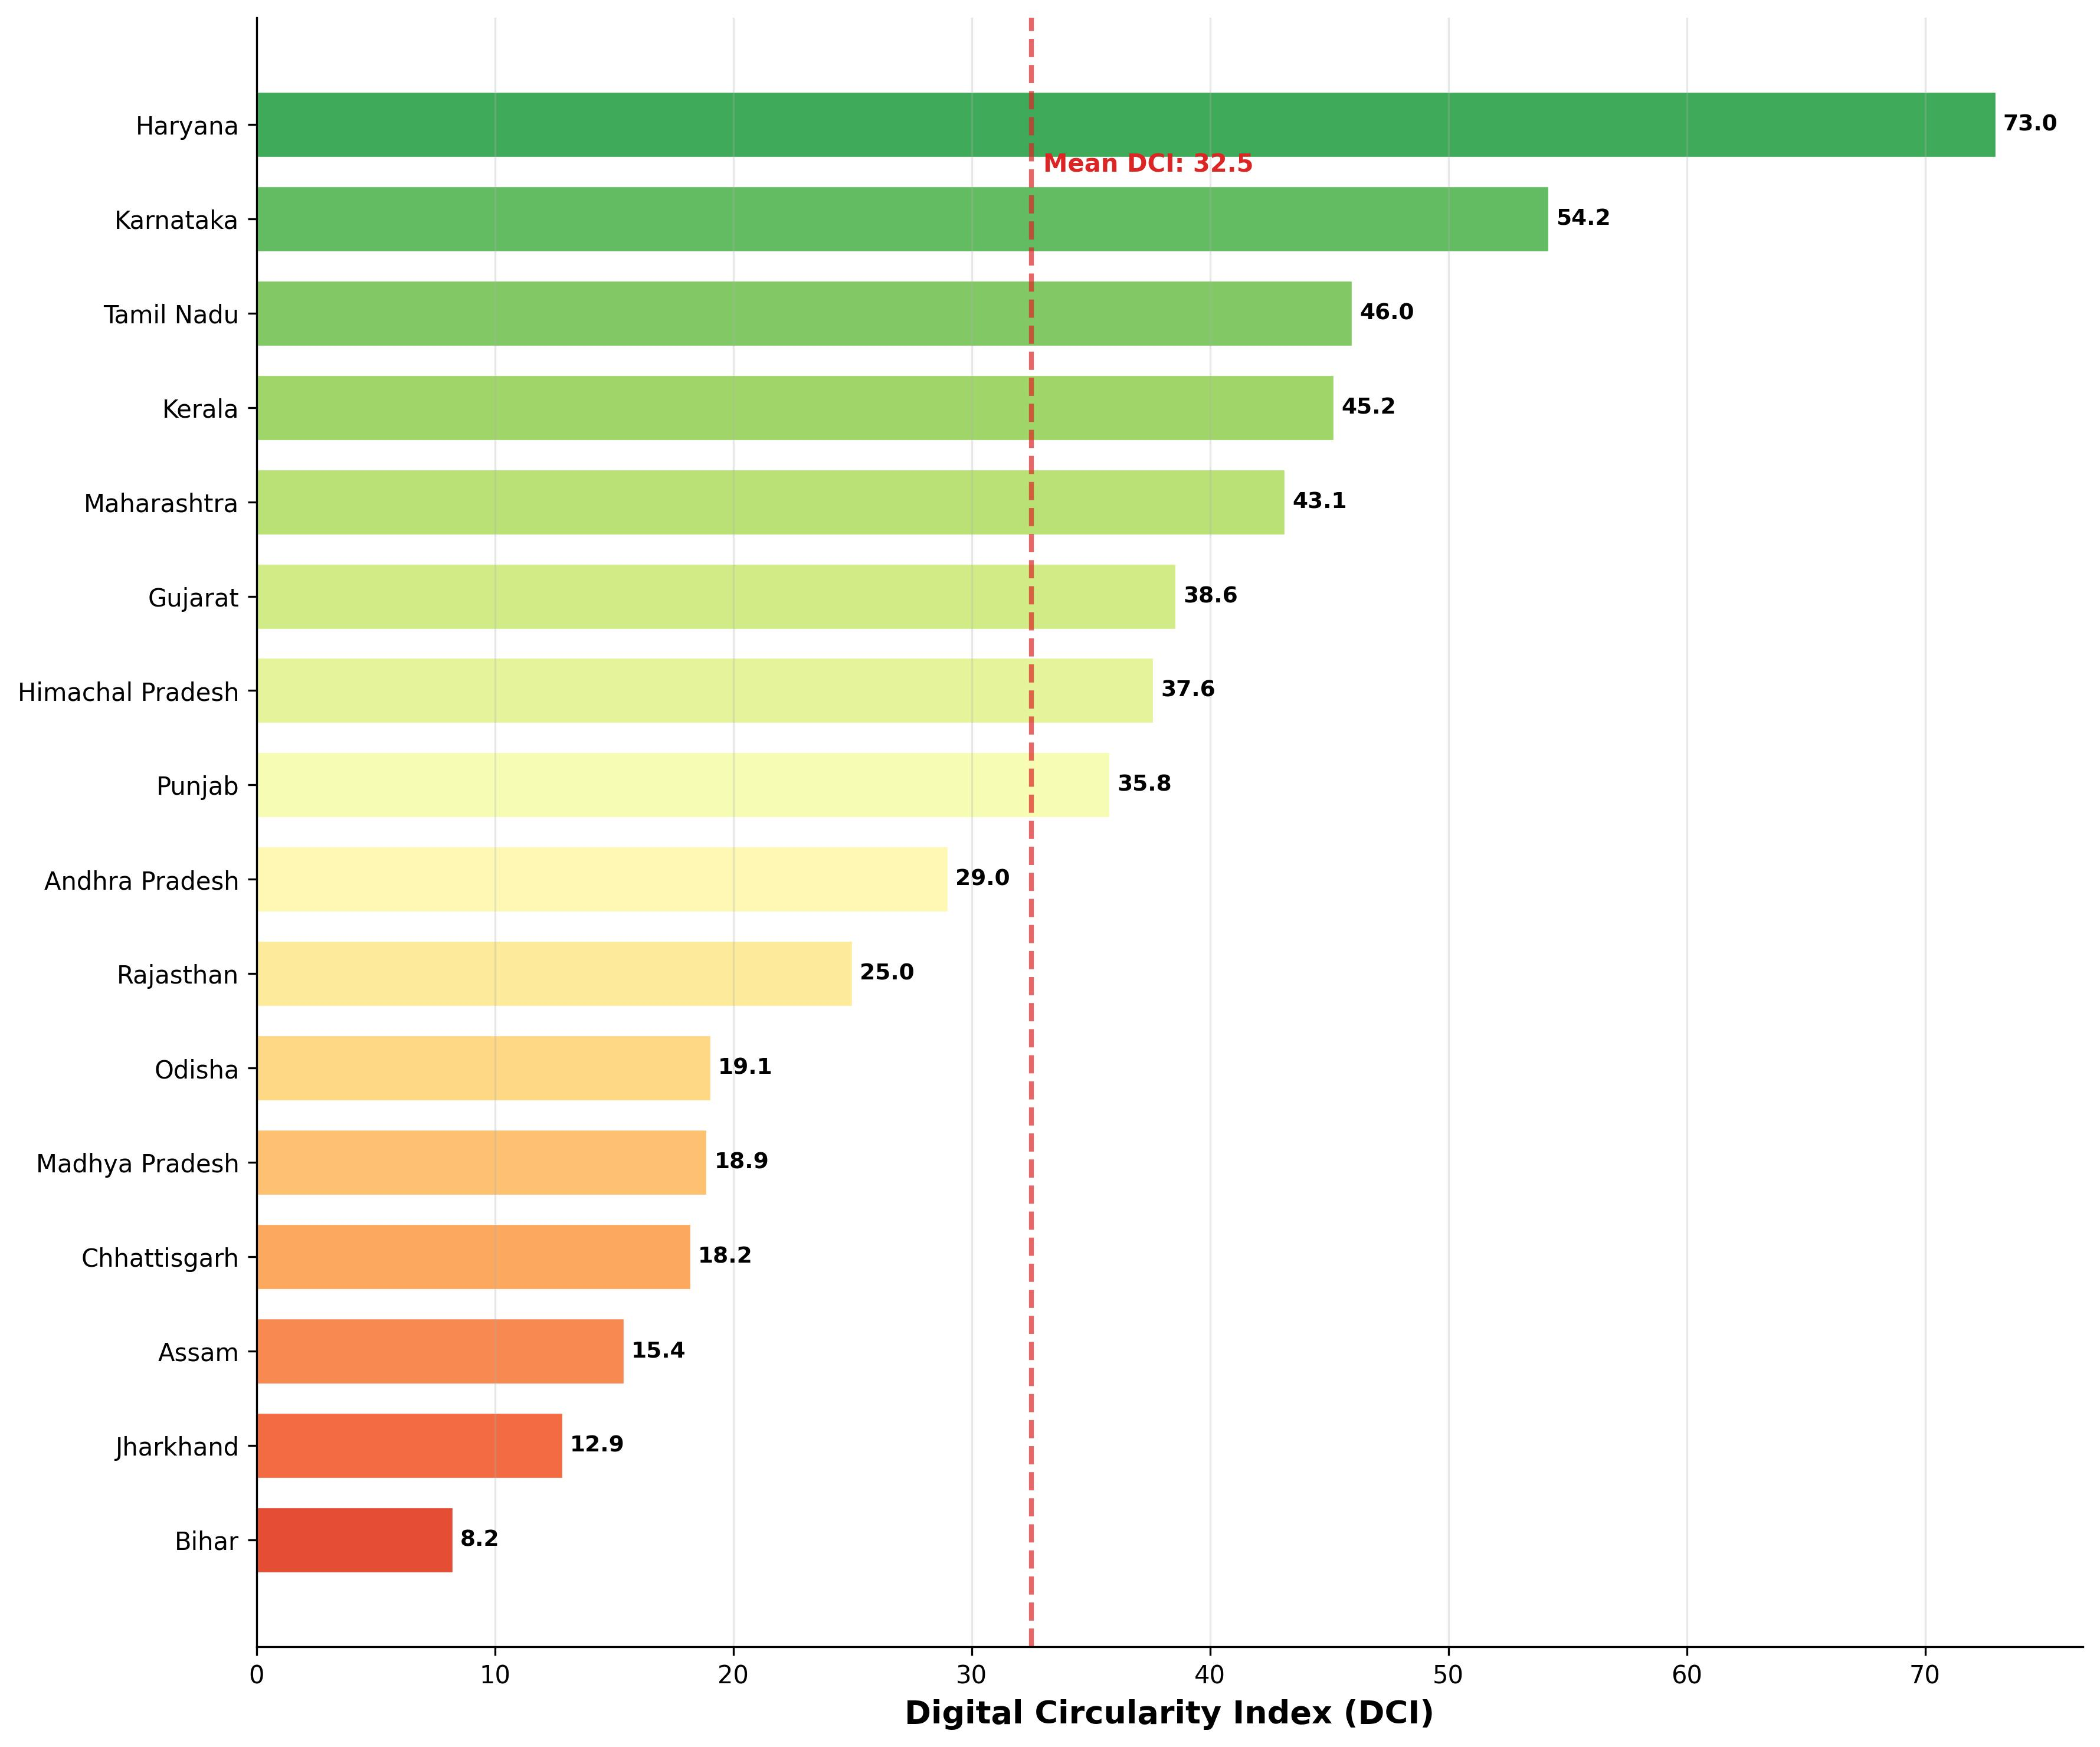
\includegraphics[width=0.82\textwidth]{figures/fig3_dci_ranking.jpg}
\caption{Digital Circularity Index ranking across 16 Indian states.}
\label{fig:dci_ranking_24}
\figsource{Authors' analysis based on the compiled state-level dataset}
\end{figure}

\subsection{Regression, robustness and mechanisms}

The regression confirms that the visual pattern is not only descriptive. A one-point increase in DAS is associated with a 0.551-point increase in CEBS, and the model explains 61\% of the observed variation. Figure~\ref{fig:scatter_24} shows the positive association, while Table~\ref{tab:core_results_24} summarises the main findings. The relationship remains significant under HC3 robust inference, permutation testing and rank-based correlation, which reduces concern that the result is only an artefact of distributional assumptions.

\begin{figure}[htbp]
\centering
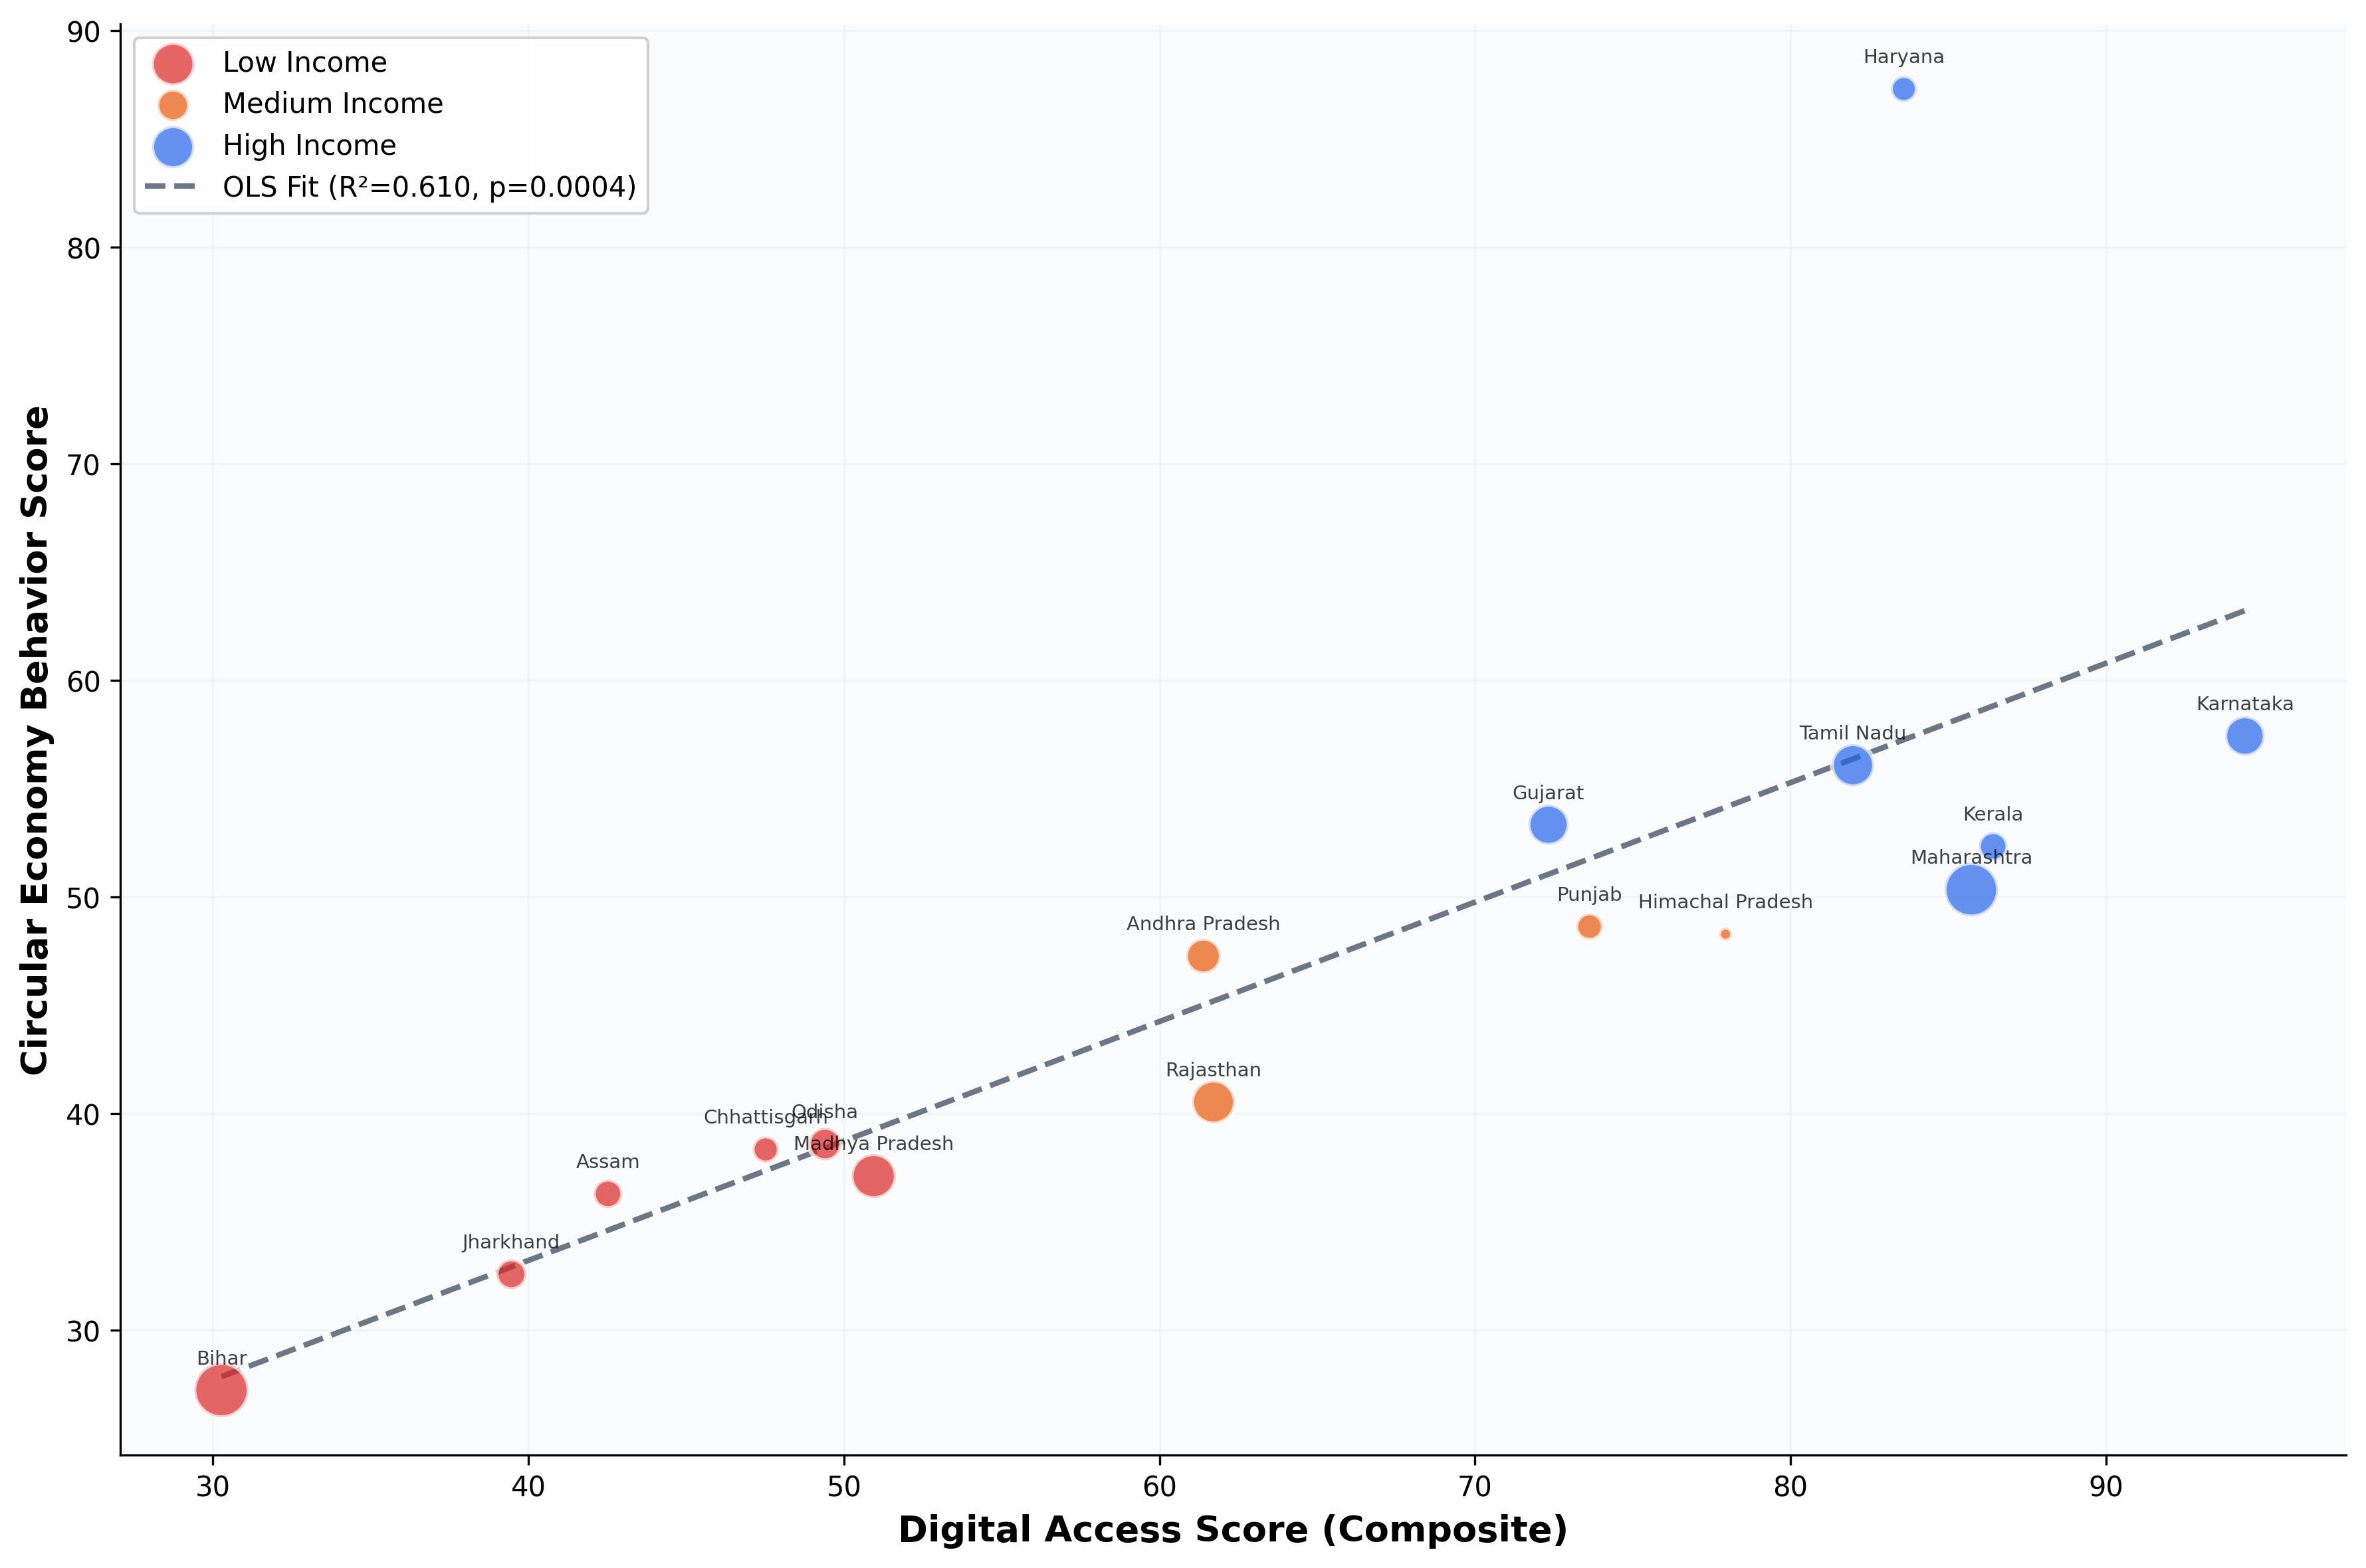
\includegraphics[width=0.75\textwidth]{figures/fig2_digital_vs_ce_scatter.jpg}
\caption{Digital Access Score and CE Behavior Score across the 16-state sample.}
\label{fig:scatter_24}
\figsource{Authors' analysis based on the compiled state-level dataset}
\end{figure}

\begin{table}[htbp]
\centering
\caption{Core Statistical Results}
\label{tab:core_results_24}
\small
\begin{tabularx}{\textwidth}{@{}>{\raggedright\arraybackslash}X>{\raggedright\arraybackslash}p{2.2cm}>{\raggedright\arraybackslash}p{3.0cm}@{}}
\toprule
\textbf{Test or Model} & \textbf{Value} & \textbf{Interpretation} \\
\midrule
OLS association (H1) & $R^2=0.610$; $\beta_1=0.551$; $p=0.000352$ & Strong positive relationship between DAS and CEBS \\
Pearson correlation & $r=0.781$ & Substantively large positive association \\
Spearman correlation & $\rho=0.912$; $p<0.001$ & Rank-order relationship remains strong \\
HC3 robust inference & $p=0.000011$ & Result remains significant under heteroskedasticity-robust errors \\
Permutation test & $p=0.0001$ & Association is unlikely under random reassignment \\
Mediation via UPI (H2) & Sobel $z=-0.241$; $p=0.810$ & No evidence that UPI mediates the main relationship \\
Threshold analysis (H3) & Breakpoint $=118.77\%$ tele-density & CE performance rises sharply up to the threshold, but evidence above it is based on very few states \\
\bottomrule
\end{tabularx}
\tabsource{Authors' analysis}
\end{table}

The UPI result is useful precisely because it is negative. Once DAS is already in the model, UPI adoption contributes little explanatory value and the indirect path is not significant. Digital access in this sample therefore appears to matter less as payment activity and more as a wider infrastructure and capacity condition. By contrast, the threshold analysis offers qualified support for H3. CE performance improves up to roughly 119\% tele-density, but the post-threshold slope is estimated from only a few states, so the breakpoint should be interpreted cautiously.

\subsection{Predictive validation and explainability}

The predictive analysis asks a modest question: does the same signal remain when each state is held out in turn? In standard leave-one-out cross-validation, ElasticNet performs best among the digital-only models ($R^2=0.364$), while Lasso performs best in the full-feature comparison ($R^2=0.568$). Under the stricter nested leave-one-out setup, XGBoost achieves the strongest leak-free result ($R^2=0.511$), narrowly outperforming Random Forest. SHAP analysis then points to tele-density and per capita NSDP as the two most influential variables, while UPI contributes much less. Figure~\ref{fig:shap_24} visualises that pattern, and Table~\ref{tab:ml_results_24} summarises the predictive, explainability and clustering results.

\begin{figure}[htbp]
\centering
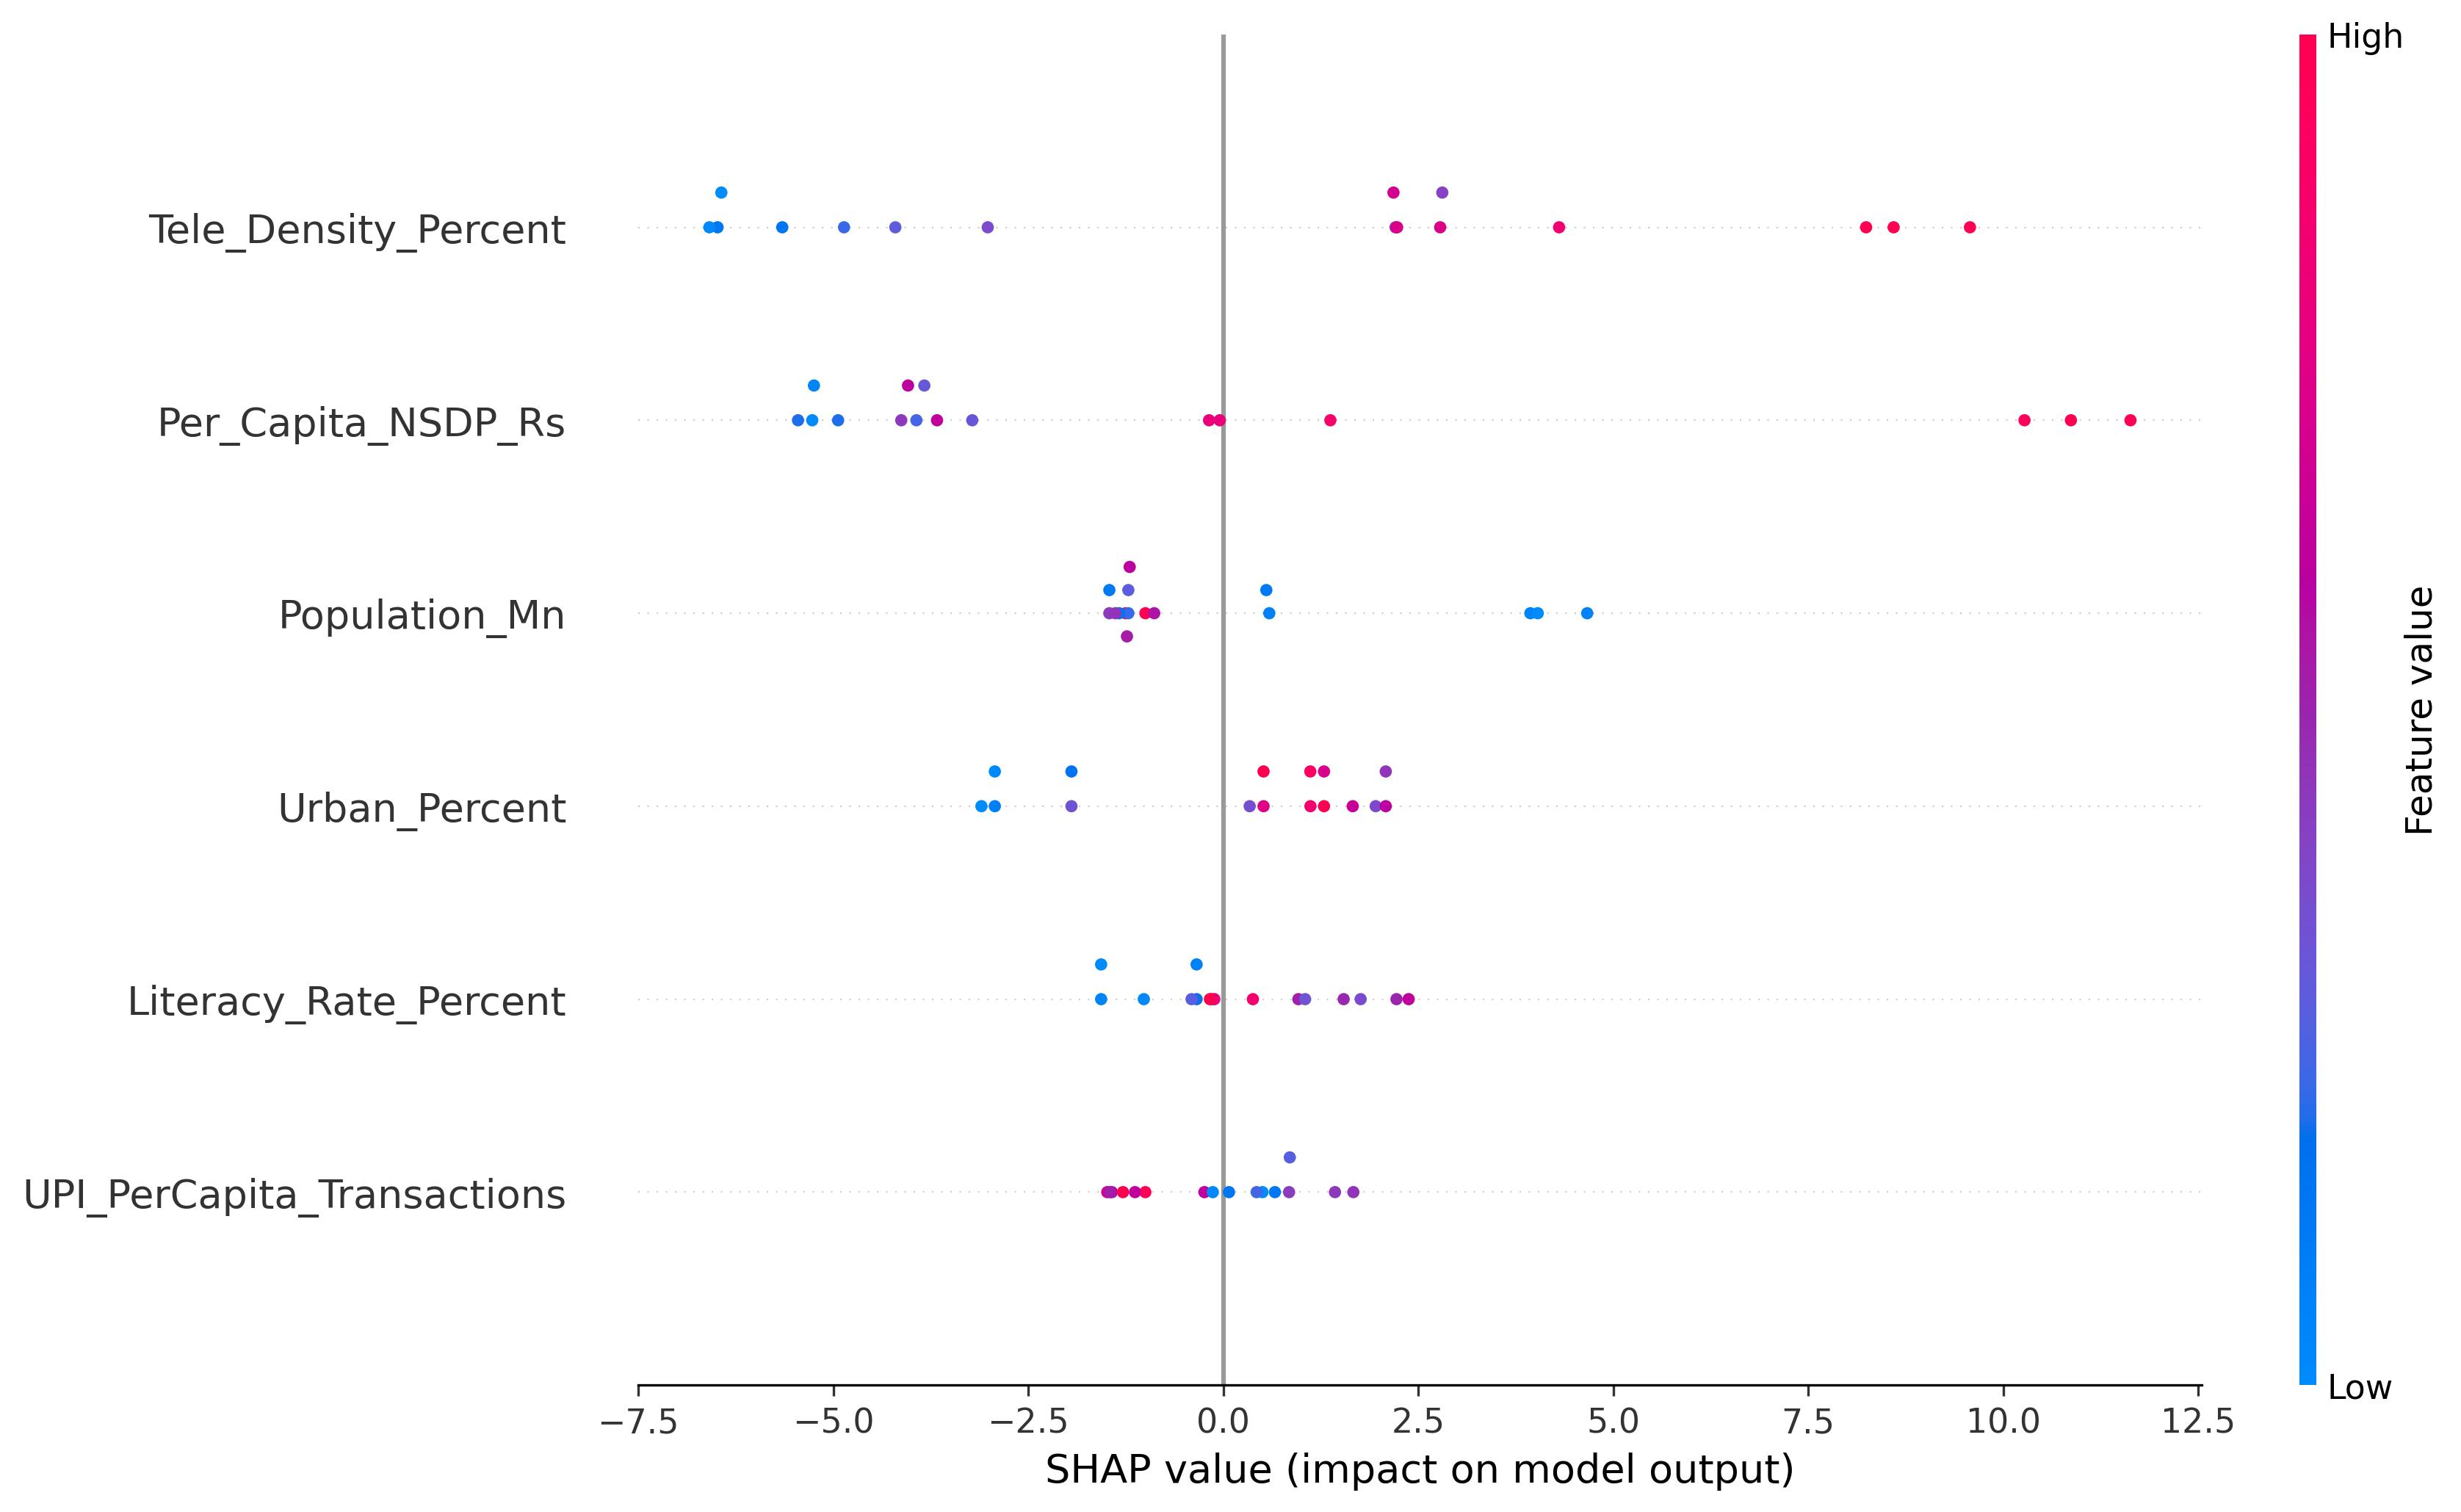
\includegraphics[width=0.80\textwidth]{figures/fig17_shap_beeswarm.jpg}
\caption{SHAP beeswarm plot for the nested XGBoost model.}
\label{fig:shap_24}
\figsource{Authors' analysis}
\end{figure}

\begin{table}[htbp]
\centering
\caption{Predictive, Explainability and Clustering Summary}
\label{tab:ml_results_24}
\small
\begin{tabularx}{\textwidth}{@{}>{\raggedright\arraybackslash}X>{\raggedright\arraybackslash}p{2.5cm}>{\raggedright\arraybackslash}X@{}}
\toprule
\textbf{Analysis} & \textbf{Key Result} & \textbf{Interpretation} \\
\midrule
Best digital-only LOO-CV model & ElasticNet, $R^2=0.364$ & Digital-access variables alone retain meaningful out-of-sample predictive value \\
Best full-model LOO-CV model & Lasso, $R^2=0.568$ & Predictive performance remains close to the main OLS result \\
Best nested LOO-CV model & XGBoost, $R^2=0.511$ & Main signal survives stricter leak-free evaluation \\
Top SHAP drivers & Tele-density; per capita NSDP & Infrastructure and economic capacity dominate the model explanation \\
K-Means typology & Two clusters; mean DCI 46.7 vs.\ 18.3 & States separate into digital leaders and emerging states with a large circularity gap \\
Extended-sample check & $n=21$; $r=0.963$ & Removing e-waste from CEBS strengthens rather than weakens the pattern \\
\bottomrule
\end{tabularx}
\tabsource{Authors' analysis}
\end{table}

The clustering result gives the statistics a more practical reading. Rather than a neat national continuum, the data point to two broad development settings. One cluster combines higher digital access with stronger CE outcomes, while the other remains weaker on both. This supports the view that digital infrastructure, administrative capacity and sustainability behavior are linked in practice. It also reinforces the point from the mediation test: tele-density matters more than digital payments alone.

\subsection{Implications and limitations}

The policy implication is not that connectivity automatically produces circularity. The more careful reading is that digital inclusion and CE strategy should not be planned as isolated domains. In lagging states, connectivity investment may also work as environmental capacity-building if it improves reporting, traceability, service delivery and administrative coordination. The study is still limited by its small cross-sectional sample, the use of 2011 Census controls, the inclusion of NSDP in both composite scores and the compression of within-state variation into state averages. The results therefore establish a consistent association, not a causal effect. Future work should extend the framework using district-level or panel data and broader circular-economy indicators.

\section{Conclusion}

This paper develops a Digital Circularity Index for 16 Indian states and finds a consistent association between digital access and circular-economy behavior. The result appears in regression, robustness checks, predictive validation and explainability analysis. Tele-density and economic capacity carry the strongest signal, while UPI adoption does not mediate the main relationship. The main lesson is therefore narrower, but more useful: digital inclusion should be understood not only as a communications or payments issue, but also as part of the institutional base on which better sustainability administration can be built.

\section*{Acknowledgment}

The authors acknowledge the Telecom Regulatory Authority of India, the Reserve Bank of India, NITI Aayog, the National Payments Corporation of India, the Central Pollution Control Board and the Census of India for maintaining the public datasets used in this study.

\clearpage
\setlength{\bibsep}{0pt}
\begingroup
\small
\begin{spacing}{2}
\begin{thebibliography}{00}

\bibitem[Avgerou(2010)]{avgerou2010}
Avgerou, C. (2010) `Discourses on ICT and development', \textit{Information Technologies \& International Development}, 6(3), pp. 1--18.

\bibitem[Baron and Kenny(1986)]{baron1986}
Baron, R.M. and Kenny, D.A. (1986) `The moderator-mediator variable distinction in social psychological research: Conceptual, strategic, and statistical considerations', \textit{Journal of Personality and Social Psychology}, 51(6), pp. 1173--1182.

\bibitem[CPCB(2023)]{cpcb2023}
CPCB (2023) \textit{Annual Report on Implementation of E-Waste (Management) Rules, 2016 for FY 2021--22} [online]. New Delhi: Central Pollution Control Board. Available at: \url{https://cpcb.nic.in/e-waste/} (Accessed: 23 April 2026).

\bibitem[Ellen MacArthur Foundation(2013)]{emf2013}
Ellen MacArthur Foundation (2013) \textit{Towards the Circular Economy: Economic and Business Rationale for an Accelerated Transition}. Cowes: Ellen MacArthur Foundation.

\bibitem[Geissdoerfer et al.(2017)]{geissdoerfer2017}
Geissdoerfer, M., Savaget, P., Bocken, N.M.P. and Hultink, E.J. (2017) `The circular economy: a new sustainability paradigm?', \textit{Journal of Cleaner Production}, 143, pp. 757--768.

\bibitem[Heeks(2017)]{heeks2017}
Heeks, R. (2017) \textit{Information and Communication Technology for Development (ICT4D)}. Abingdon: Routledge.

\bibitem[Lundberg and Lee(2017)]{lundberg2017}
Lundberg, S.M. and Lee, S.-I. (2017) `A unified approach to interpreting model predictions'. In: \textit{Advances in Neural Information Processing Systems}, 30.

\bibitem[Ministry of Electronics \& IT(2023)]{meity2023}
Ministry of Electronics \& IT (2023) \textit{Digital India Programme: Progress and Initiatives} [online]. Available at: \url{https://digitalindia.gov.in} (Accessed: 23 April 2026).

\bibitem[Mishra et al.(2025)]{icrier2025}
Mishra, D., Reddy, A., Gupta, S. and Bharti, J. (2025) \textit{State of India's Digital Economy: A Subnational Perspective, 2025} [online]. New Delhi: Indian Council for Research on International Economic Relations. Available at: \url{https://icrier.org/publications/state-of-indias-digital-economy-a-subnational-perspective-2025/} (Accessed: 27 April 2026).

\bibitem[NITI Aayog(2021)]{nitiCE2021}
NITI Aayog (2021) \textit{Circular Economy in India: Rethinking Growth for Long-Term Prosperity}. New Delhi: Government of India.

\bibitem[NITI Aayog(2024)]{nitiSDG2024}
NITI Aayog (2024) \textit{SDG India Index \& Dashboard 2023--24}. 4th edn [online]. New Delhi: Government of India. Available at: \url{https://sdgindiaindex.niti.gov.in} (Accessed: 23 April 2026).

\bibitem[NPCI(2025)]{npci2025}
NPCI (2025) \textit{UPI Product Statistics (Monthly)} [online]. Mumbai: National Payments Corporation of India. Available at: \url{https://www.npci.org.in/what-we-do/upi/product-statistics} (Accessed: 23 April 2026).

\bibitem[Sch\"oggl et al.(2023)]{schoggl2023}
Sch\"oggl, J.-P., Rusch, M., Stumpf, L. and Baumgartner, R.J. (2023) `Implementation of digital technologies for a circular economy and sustainability management in the manufacturing sector', \textit{Sustainable Production and Consumption}, 35, pp. 401--420. doi: \url{https://doi.org/10.1016/j.spc.2022.11.012}.

\bibitem[TRAI(2024)]{trai2024}
TRAI (2024) \textit{Indian Telecom Services Performance Indicators Report: April--June 2024} [online]. New Delhi: Telecom Regulatory Authority of India. Available at: \url{https://www.trai.gov.in/sites/default/files/2024-09/IndicatorReport1oct09.pdf} (Accessed: 23 April 2026).

\end{thebibliography}
\end{spacing}
\endgroup

\end{document}
